\section{Dynamic Memory Allocation}
\label{sec:malloc}
\begin{frame}<beamer>
    \frametitle{Outline}
    \tableofcontents[currentsection]
\end{frame}

\begin{frame}[fragile]{Static and Dynamic Memory Allocation (1)}
\begin{itemize}
	\item {Recall what the variables we learned so far}
	\begin{enumerate}
		\item {Primitive type variables}
		\item {Primitive type arrays}
		\item {Composite type variables}
		\item {Composite type arrays}
	\end{enumerate}
\end{itemize}
\begin{lstlisting}[xleftmargin=0.32\linewidth, linewidth=0.6\linewidth]
struct STD {
  char name[16];
  float gpa;
};
typedef STD STDT;
int main()
{
   int a, a1[10];
   STDT b, b1[10];
}
\end{lstlisting}
\vspace{-0.1in}
\begin{itemize}
	\item {The memory cells for a, a1, b and b1 are allocated when your code is loaded into memory}
	\item {It is done \textcolor{red}{before the code is executed}}
\end{itemize}
\end{frame}

\begin{frame}[fragile]{Static and Dynamic Memory Allocation (2)}
\begin{itemize}
	\item {In some cases, we are not sure how long is the array we need before run it}\
	\item {We have two options for this case}
	\begin{enumerate}
		\item {Apply for a very long array, i.e., 65,536}
		\item {Apply the memory cells in the \textcolor{red}{runtime}}
	\end{enumerate}
	\item {The second way is called dynamic memory allocation}
\end{itemize}

\end{frame}

\begin{frame}[fragile]{Dynamic Memory Allocation: grammar (1)}
\begin{center}
\Large{
  \textcolor{blue}{int} *p = (\textcolor{blue}{int}*)malloc(\textcolor{blue}{sizeof}(\textcolor{blue}{int})*10);
}
\end{center}
\vspace{0.2in}
\begin{enumerate}
	\item {Apply a block of memory sized of 10*sizeof(int)=??}
	\item {Function ``\textbf{malloc}($\cdot$)'' returns the starting address of this memory}
	\item {Convert this starting address to an \textcolor{blue}{int} type pointer}
	\item {Assign this starting address to \textbf{p}}
\end{enumerate}
\end{frame}

\begin{frame}[fragile]{Dynamic Memory Allocation: grammar (2)}
\begin{center}

\Large{
  \textcolor{blue}{int} *p = (\textcolor{blue}{int}*)malloc(\textcolor{blue}{sizeof}(\textcolor{blue}{int})*10);
}

\end{center}
\vspace{0.2in}
\begin{enumerate}
	\item {Function ``\textbf{malloc}($\cdot$)'' sends the applicaiton to OS}
	\item {When the application is approved, a block of memory is returned}
	\item {OS extracts memory from \textbf{Heap}}
	\item {Once it is allocated, you can operate it as an array}
\end{enumerate}
\end{frame}

\begin{frame}[fragile]{Dynamic Memory Allocation: explained}
\vspace{-0.1in}
\begin{figure}
\begin{center}
	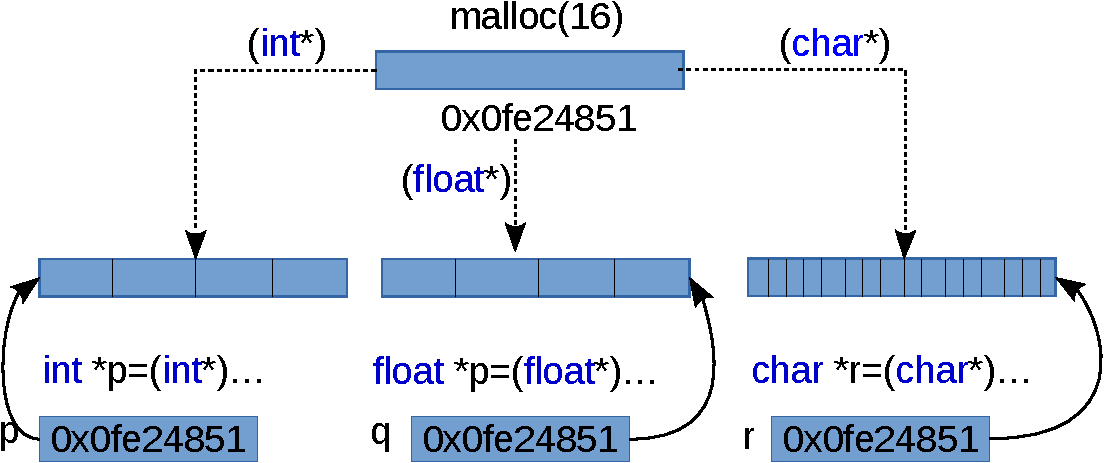
\includegraphics[width=0.8\linewidth]{figs/malloc.pdf}
\end{center}
\end{figure}
\vspace{-0.1in}
\begin{columns}
\begin{column}{0.45\linewidth}
\begin{lstlisting}
#include <stdlib.h>
int main()
{
    void *x = malloc(16);
    int *p = (int*)x;
    float *q = (float*)x;
    char *r = (char*)x;
}
\end{lstlisting}
\end{column}
\begin{column}{0.5\linewidth}
\begin{itemize}
	\item {We \textcolor{red}{just show it is possible}}
	\item {It is \textcolor{red}{NOT} suggested in practice}
\end{itemize}
\end{column}
\end{columns}
\end{frame}

\begin{frame}[fragile]{Dynamic Memory Allocation: example}
\begin{columns}
\begin{column}{0.85\linewidth}
\begin{lstlisting}
#include <stdlib.h>
int main()
{
   int i = 0, *a1 = (int*)malloc(5*sizeof(int));
   for(i = 0; i < 5; i++)
   {
       a1[i] = i+1;
   }
   free(a1);//<--release the memory pointing by a1
   return 0;
}
\end{lstlisting}
\end{column}
\end{columns}
\vspace{-0.2in}
\begin{enumerate}
	\item {Function ``\textbf{malloc}($\cdot$)'' returns the starting address of this block of memory}
	\item {Once it is allocated, you can operate it as an array}
	\item {Always remember to \textcolor{red}{release} it by calling free($\cdot$)}
\end{enumerate}
\end{frame}

\begin{frame}[fragile]{Dynamic Memory Allocation: memory leakage (1)}
\begin{itemize}
	\item {Different from static memory allocation}
	\item {You are required to release the dynamically allocated memory on your own}
	\item {If you fail to do that, memory leakage occurs (90\%) C bugs arise from this}
\end{itemize}
\begin{columns}
\begin{column}{0.8\linewidth}
\begin{lstlisting}
#include <stdlib.h>
int main()
{
   int i = 0, *a1 = (int*)malloc(5*sizeof(int));
   for(i = 0; i < 5; i++)
   {
       a1[i] = i+1;
   }
   free(a1);//<-- very important here
   return 0;
}
\end{lstlisting}
\end{column}
\end{columns}
\end{frame}

\begin{frame}[fragile]{Dynamic Memory Allocation: memory leakage (2)}
\begin{columns}
\begin{column}{0.8\linewidth}
\begin{lstlisting}
#include <stdlib.h>
int main()
{
   int i = 0, *a1 = (int*)malloc(5*sizeof(int));
   for(i = 0; i < 5; i++)
   {
       a1[i] = i+1;
   }
   free(a1);
   a1[2] = 3;//<--- illegal memory access
   return 0;
}
\end{lstlisting}
\end{column}
\end{columns}
\begin{itemize}
	\item {You are not allowed to use memory that has been released}
	\item {Above code (line 10) causes \textcolor{red}{illegal memory access exception}}
\end{itemize}
\end{frame}

\begin{frame}[fragile]{Dynamic Memory Allocation: memory leakage (3)}

\begin{lstlisting}, xleftmargin=0.02\linewidth, linewidth=0.98\linewidth]
#include <stdlib.h>
int main()
{
   int i = 0, *a1 = (int*)malloc(5*sizeof(int));
   for(i = 0; i < 5; i++)
   {
       a1[i] = i+1;
   }
   a1 = (int*)malloc(15*sizeof(int));//<-something wrong here
   free(a1);
   return 0;
}
\end{lstlisting}

\vspace{-0.15in}
\begin{itemize}
	\item {You are not allowed to use memory that has been released}
	\item {We lose the pointer to one block of memory (at line 9)}
	\item {Memory leaks (\textcolor{red}{ghost} memory cells)}
\end{itemize}
\end{frame}


